\documentclass[12pt]{article}
    \usepackage{amsthm,amsmath,amssymb}
    \usepackage{amsfonts}
    \usepackage{mathrsfs}
    \usepackage{listings}
    \usepackage{verbatim}
    \usepackage{fancyhdr}
    \usepackage{graphicx}
    \usepackage{xeCJK}
    \usepackage{xcolor}      %代码着色宏包
    \usepackage{CJK}         %显示中文宏包
    \usepackage{fontspec}
    \usepackage{float}
    \usepackage{placeins}
    \usepackage{subfigure}
    \usepackage{bm}
    \usepackage[colorlinks,linkcolor=blue]{hyperref}

\lstset{
    basicstyle=\fontspec{Consolas},
    %numbers=left,
    %rulesepcolor=\color{red!20!green!20!blue!20},
    escapeinside=``,
    xleftmargin=2em,xrightmargin=2em, aboveskip=1em,
    %背景框
    framexleftmargin=1.5mm,
    frame=shadowbox,
    %背景色
    backgroundcolor=\color[RGB]{245,245,244},
    %样式
    keywordstyle=\color{blue}\fontspec{Consolas Bold},
    %identifierstyle=\bf,
	breaklines=true,
    numberstyle=\color[RGB]{0,192,192},
    commentstyle=\color[RGB]{96,96,96}\fontspec{Consolas Italic},
    stringstyle=\rmfamily\slshape\color[RGB]{128,0,0},
    %显示空格
    showstringspaces=false
}

\textheight 23cm \textwidth 15cm
\topmargin -1.5cm \oddsidemargin 0.3cm \evensidemargin -0.3cm

\begin{document}
\title {Assignment-matlab 1}
\date{\today}
\author{Haowei Kan}
\maketitle
\section{Introduction}
The term "image warping" describes methods for deforming images to arbitrary shapes. The problem of image deformation can be formulated as follows:

{\bf Input:} n pairs $(\mathbf{p}_i,\mathbf{q}_i) $ of control points, $\mathbf{p}_i,\mathbf{q}_i\in \mathbb{R}^2, i = 1,...,n $.

{\bf Output:} An at least continuous function $\mathbf{f}:\mathbb{R}^2\rightarrow\mathbb{R}^2$ with $\mathbf{f}(\mathbf{p}_i)=\mathbf{q}_i,i = 1,...,n$.

\noindent The interpolation problem of scattered data of two variables can be formulated as:

{\bf Input:} n data points $(\mathbf{x}_i,y_i),\mathbf{x}_i\in\mathbb{R}^2,y_i\in\mathbb{R},i=1,...,n$

{\bf Output:} An at least continuous function $f:\mathbb{R}^2\rightarrow\mathbb{R}$ interpolating the given data points, i.e.$f(\mathbf{x}_i)=y_i, i=1,...,n$.

\noindent So we can solve the image deformation problem by treating each component of target points separately and then the interpolation can be used for it. Here we will introduce two image warping alogrithms based on this idea.


\section{Algorithms}
\subsection{Inverse Distance Weighted Interpolation Methods}
For each data point $\mathbf{p}_i$, a local approximation $f_i(\mathbf{p}):\mathbb{R}^2\rightarrow\mathbb{R}$ with $f_i(\mathbf{p}_i)=y_i, i=1,...,n$ is determined. The interpolation function is a weighted average of these local approximations, with weights dependent on the distance of the observed point from the given data points,
\begin{equation}
    f(\mathbf{p})=\sum_{i=1}^nw_i(\mathbf{p})f_i(\mathbf{p})
\end{equation}
where $f_i(\mathbf{p}_i)=y_i,i=1,...,n.$  $w_i:\mathbb{R}^2\rightarrow\mathbb{R}$ is the weight function, which must satisfy the conditions
\begin{equation}
    w_i(\mathbf{p}_i)=1,\ \ \sum_{i=1}^nw_i(\mathbf{p})=1,\ \ \mathrm{and}\ w_i(\mathbf{p})\ge0, i=1,...,n
\end{equation}
The application of inverse distance-weighted interpolation to image warping gives
\begin{equation}
    \mathbf{f}(\mathbf{p})=\sum_{i=1}^nw_i(\mathbf{p})\mathbf{f}_i(\mathbf{p})
\end{equation}
where $\mathbf{f}(\mathbf{p}_i)=\mathbf{q}_i,i=1,...,n$. $\mathbf{f}_i:\mathbb{R}^2\rightarrow\mathbb{R}^2$ are the local approximations.


\subsubsection*{weight function}
A simple weight function is proposed by Shepard, which is
\begin{equation}
    \displaystyle w_i(\mathbf{p})=\frac{\sigma_i(\mathbf{p})}{\sum\limits_{j=1}^n\sigma_j(\mathbf{p})}\ \mathrm{with}\ \sigma_i(\mathbf{p})=\frac{1}{d(\mathbf{p},\mathbf{p}_i)^\mu}\label{con:inventoryflow}
\end{equation}
where $d(\mathbf{p},\mathbf{p}_i)$ is the distance between $\mathbf{p}$ and $\mathbf{p}_i$.

The smoothness is determined by the exponent $\mu$. $\mu>1$ assures continuity of the derivatives.
\subsubsection*{local approximation}
For the local approximations, linear or quadratic polynomials are normally used. We used the linear polynomials in our experiments, i.e.
\begin{equation}
    \mathbf{f}_i(\mathbf{p})=\mathbf{q}_i+\mathbf{T}_i(\mathbf{p}-\mathbf{p}_i)
\end{equation}

We compute T by minimizing the squared error of the mapping of other nearby control points $\mathbf{p}_j$ with $f_i$, weighted with the $\sigma_i(\mathbf{p}_j)$ from Equation \eqref{con:inventoryflow}. The corresponding error function $E_i(f)$ is
\begin{equation}
    E_i(T)=\sum_{j=1,j\neq i}^n\sigma_i(\mathbf{p}_j)\left\Vert\mathbf{q}_i+\left(
    \begin{array}{cc}
        t_{11} & t_{12} \\
        t_{21} & t_{22}
    \end{array}\right)(\mathbf{p}_j-\mathbf{p}_i)-\mathbf{q}_j\right\Vert^2
\end{equation}
It can be also written in the matrix form, which is
\begin{equation}
    E_i(T)=\left\Vert \tilde{P}_i T^T-\tilde{Q}_i \right\Vert_F^2
\end{equation}
where
\begin{equation}
    \begin{split}
        &P=\left(
        \begin{array}{cc}
                p_{11} & p_{12} \\
                p_{21} & p_{22} \\
                \vdots & \vdots \\
                p_{n1} & p_{n2}
            \end{array}
        \right),W_i=\left(
        \begin{array}{cccc}
                \sqrt{\sigma_i(\mathbf{p}_1)} &                               &        & 0                             \\
                                              & \sqrt{\sigma_i(\mathbf{p}_2)} &        &                               \\
                                              &                               & \ddots &                               \\
                                              &                               &        & \sqrt{\sigma_i(\mathbf{p}_n)} \\
            \end{array}
        \right),P_i=\left(
        \begin{array}{cc}
                p_{i1} & p_{i2} \\
                p_{i1} & p_{i2} \\
                \vdots & \vdots \\
                p_{i1} & p_{i2}
            \end{array}
        \right),\\
        &Q=\left(
        \begin{array}{cc}
                q_{11} & q_{12} \\
                q_{21} & q_{22} \\
                \vdots & \vdots \\
                q_{n1} & q_{n2}
            \end{array}
        \right),Q_i=\left(
        \begin{array}{cc}
                q_{i1} & q_{i2} \\
                q_{i1} & q_{i2} \\
                \vdots & \vdots \\
                q_{i1} & q_{i2}
            \end{array}
        \right),\tilde{P}_i=W_i(P-P_i),T=\left(
        \begin{array}{cc}
                t_{11} & t_{12} \\
                t_{21} & t_{22}
            \end{array}
        \right),\tilde{Q}_i=W_i(Q-Q_i)
    \end{split}
\end{equation}
The minimum of the error function is obtained with the derivative with respect to T. Setting the derivative to zero, we have
\begin{equation}
    T_i=((\tilde{P_i}^T\tilde{P}_i)^{-1}\tilde{P_i}^T\tilde{Q}_i)^T
\end{equation}
\subsubsection*{complexity analysis}
With $n$ the number of control points, we need $O(n)$ time to get matrix T. And for every pixels in the image, we need $O(n)$ time to compute the weight and get the result coordinate.So the complexity is $O(nN+n^2)$ where N is the number of pixels.


\subsection{Radial Basis Functions Methods}
Another popular approach to scattered data interpolation is to construct the interpolation function as a linear combination of basis functions, then determine the coefficients of the basis functions,
\begin{equation}
    f(\mathbf{p})=\sum_{i=1}^n\alpha_if_i(d(\mathbf{p},\mathbf{p}_i))+p_m(\mathbf{p})
\end{equation}
The values of the basis funciton $f_i$ depend only on the distance from the data point and are thus called radial. $p_m(\mathbf{p})$ is a polynomial of degree $m$.

Linear polynomials, where $m=1$, give very good results---often better than higher degree. More easily, an identical transform is usually sufficient if no strong global rotations are involved. In this experiment, we will just let $p_m$ be an identical transform, so the application of radial basis functions to the problem of deformation gives
\begin{equation}
    \mathbf{f}(\mathbf{p})=\sum_{i=1}^n\bm{\alpha}_if(d(\mathbf{p},\mathbf{p}_i))+\mathbf{p}
\end{equation}

In term of radial basis function part, the thin-plate spline, the Gaussian and the multiquadrics are all commonly used. In this experiment we will choose the multiquadrics, which is
\begin{equation}
    f(d)=(d^2+r^2)^{\mu/2}
\end{equation}
And we used individual values $r_i$ for each data points, computed from the distance to the nearest neighbor:
\begin{equation}
    r_i=\min_{i\neq j}d_i(\mathbf{p}_j)
\end{equation}
So the resulting mapping function is then
\begin{equation}
    \mathbf{f}(\mathbf{p})=\sum_{i=1}^n\bm{\alpha}_i(d(\mathbf{p},\mathbf{p}_i)^2+r_i^2)^{\mu/2}+\mathbf{p}
\end{equation}
where $\bm{\alpha}_i$ can be calculated with $\mathbf{f}(\mathbf{p}_i)=\mathbf{q}_i$ by solving 2N linear equations.
\subsubsection*{complexity analysis}
For every pixel, we need $O(n)$ time to compute the result of radial basis functions. Besides, we need another $O(n^3)$ time to get the coefficients $\alpha_i$. So it gives the complexity of $O(nN+n^3)$.

\section{Results}
\begin{figure}
    \subfigure[IDW]{
        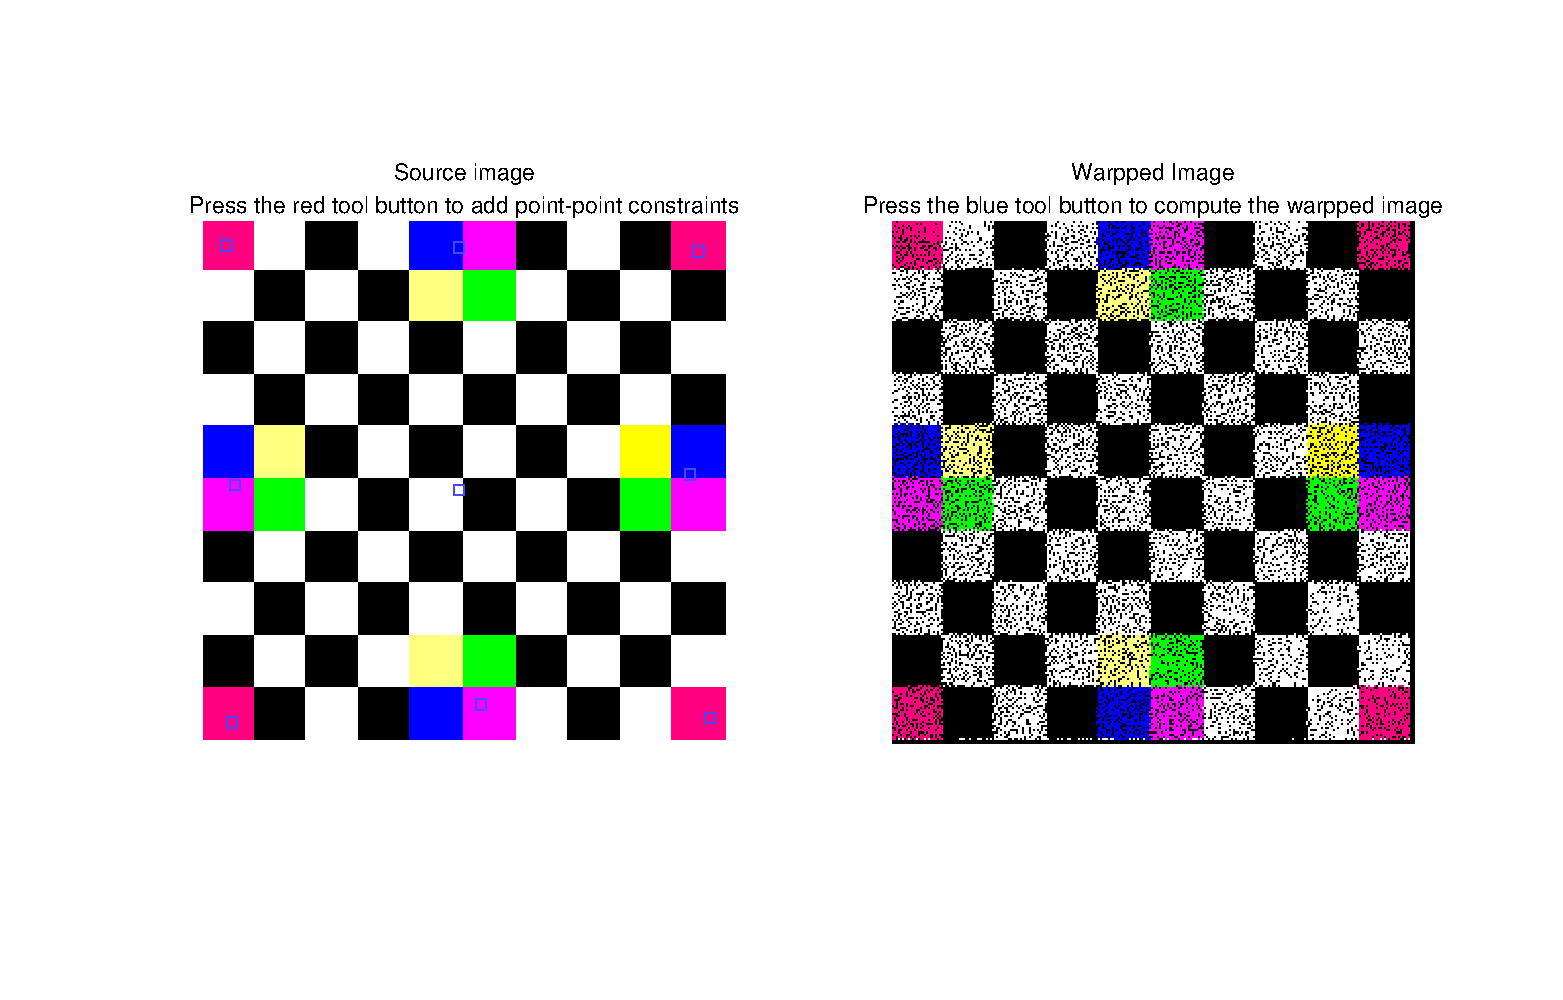
\includegraphics[width=0.5\textwidth]{ResultImage/idw3.pdf}
    }
    \subfigure[RBF]{
        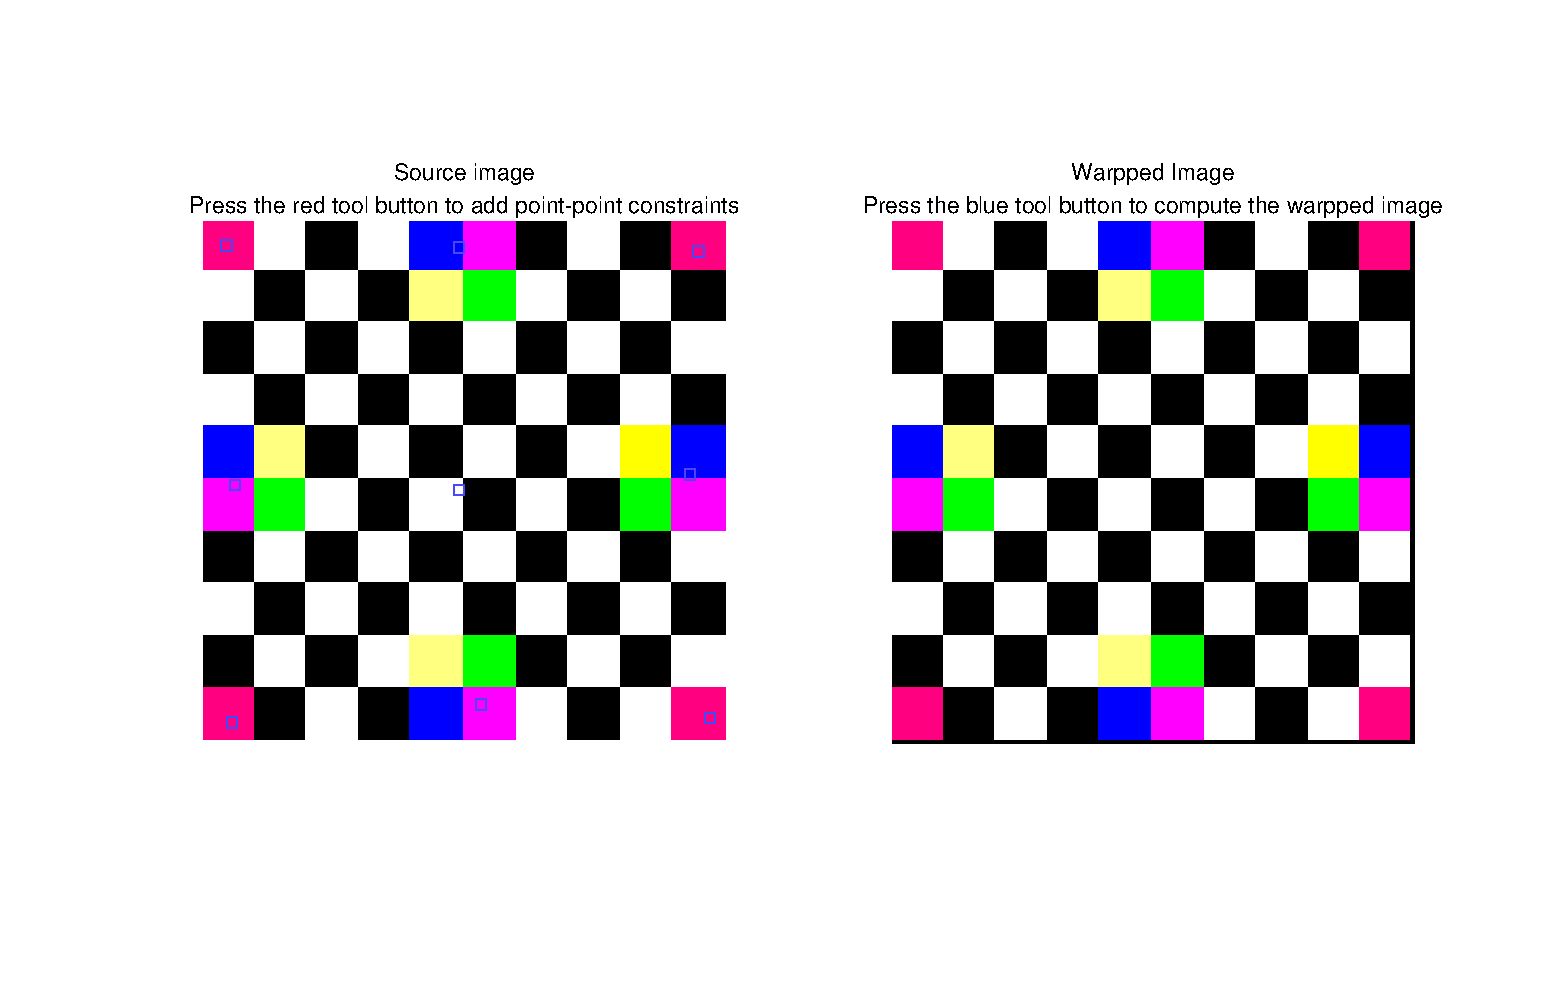
\includegraphics[width=0.5\textwidth]{ResultImage/rbf3.pdf}
    }
    %    \caption{n=9}
    %\end{figure}
    %\begin{figure}[htb]
    \subfigure[IDW]{
        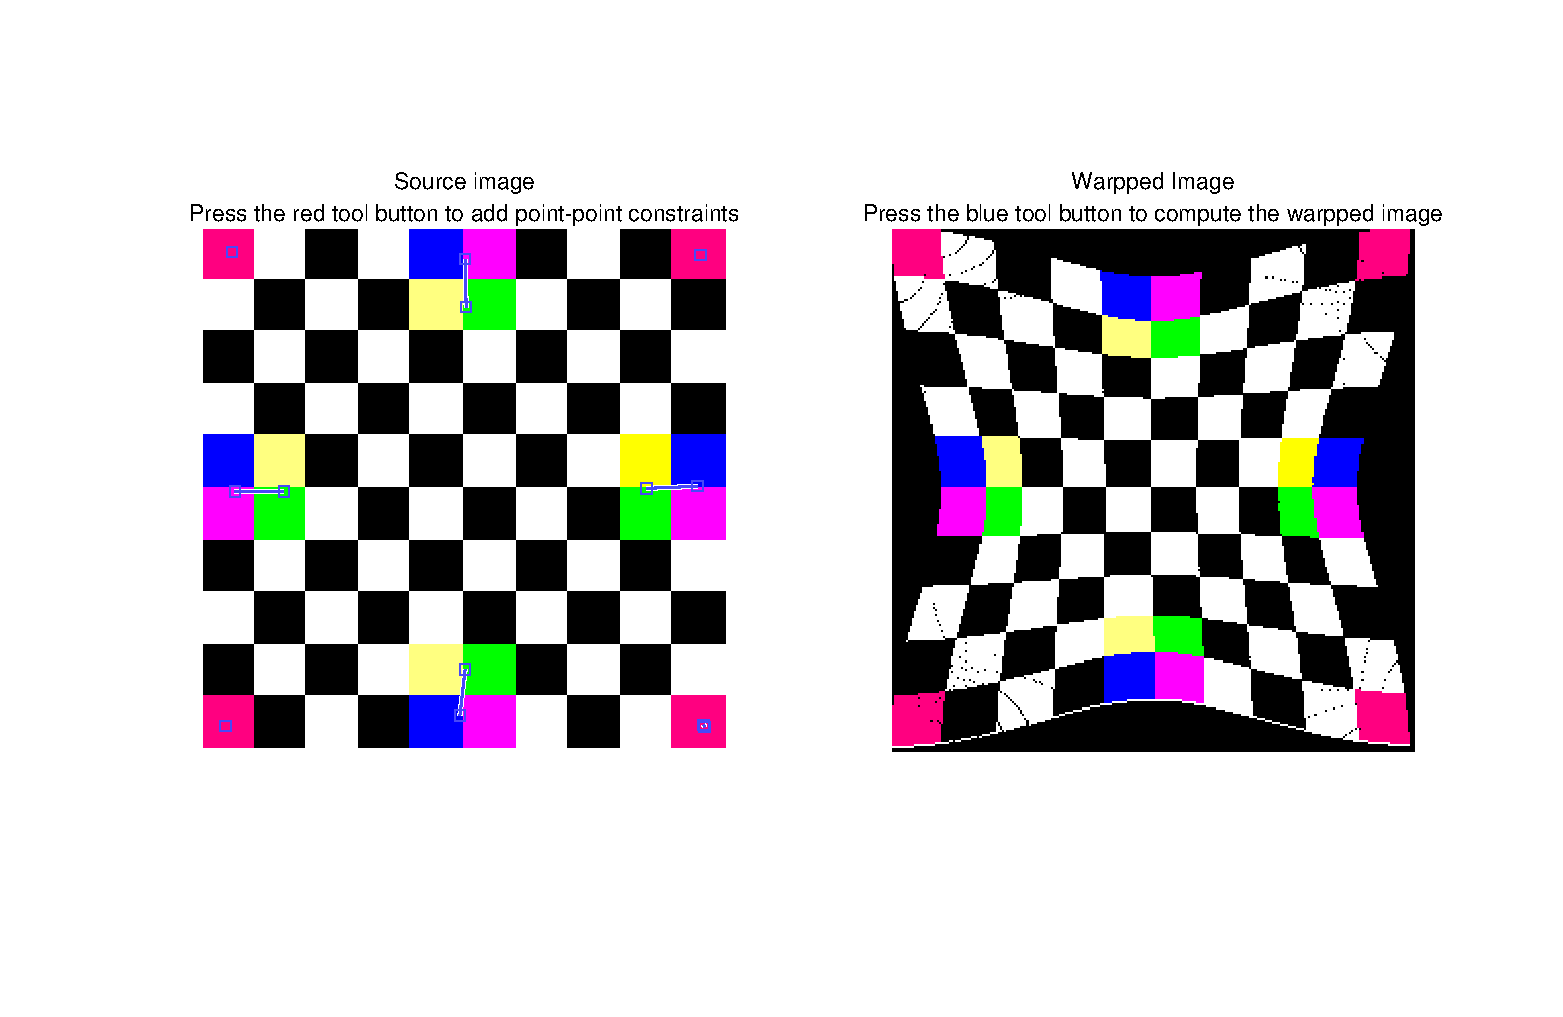
\includegraphics[width=0.5\textwidth]{ResultImage/idw1.pdf}
    }
    \subfigure[RBF]{
        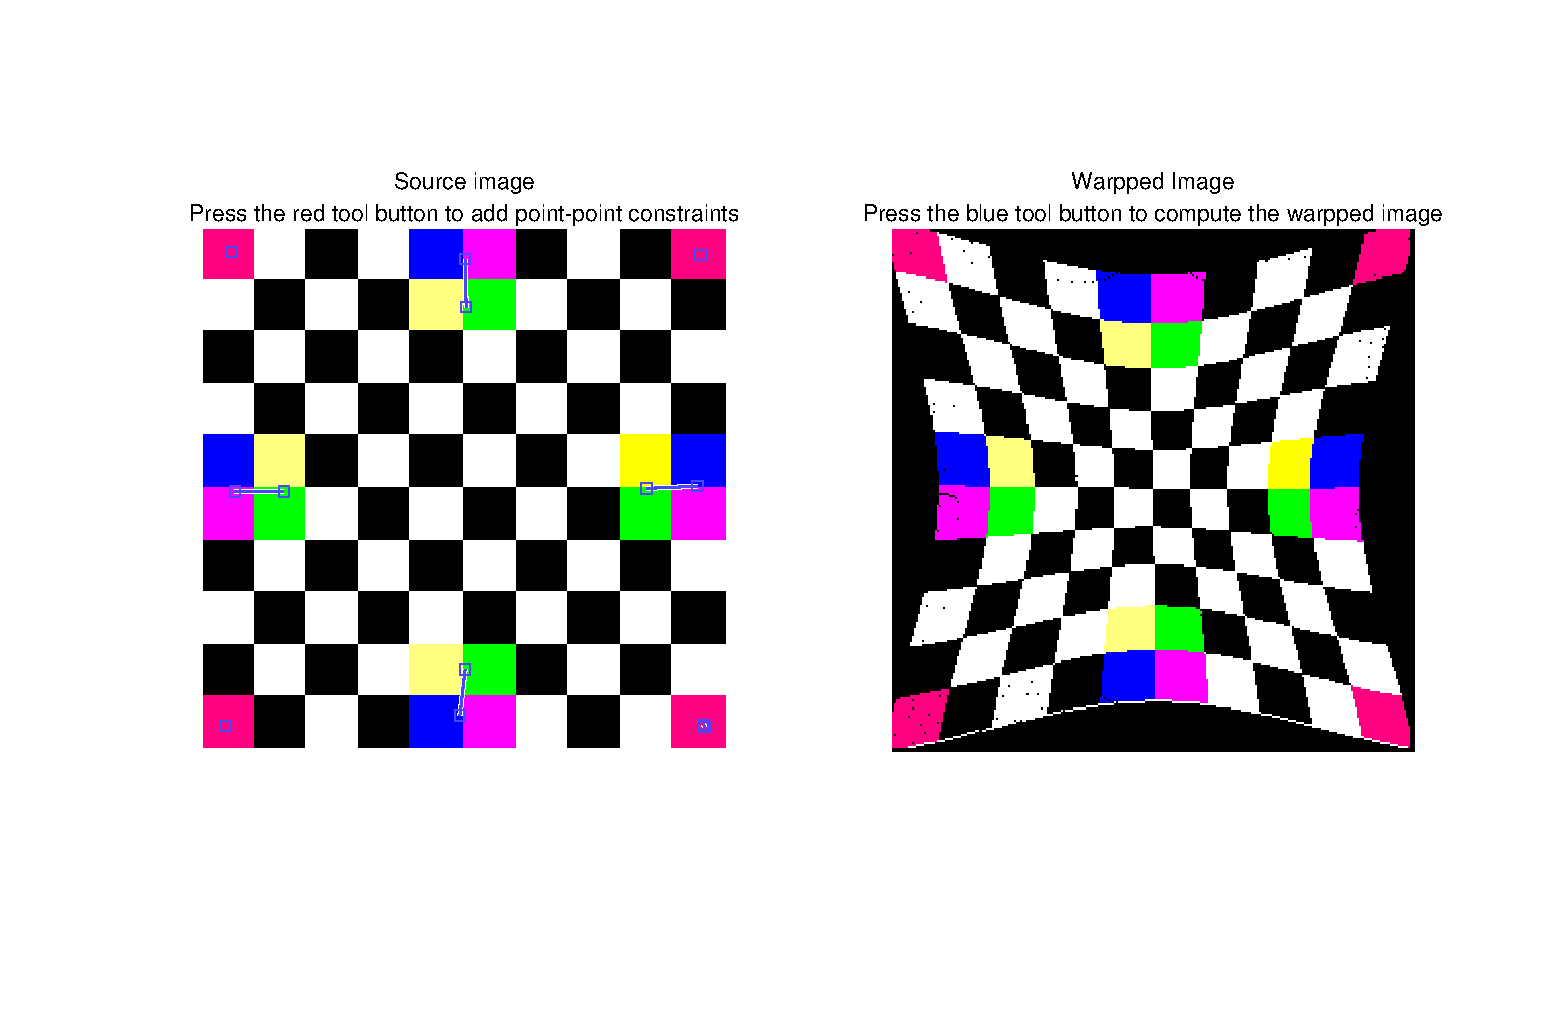
\includegraphics[width=0.5\textwidth]{ResultImage/rbf1.pdf}
    }
    \subfigure[IDW]{
        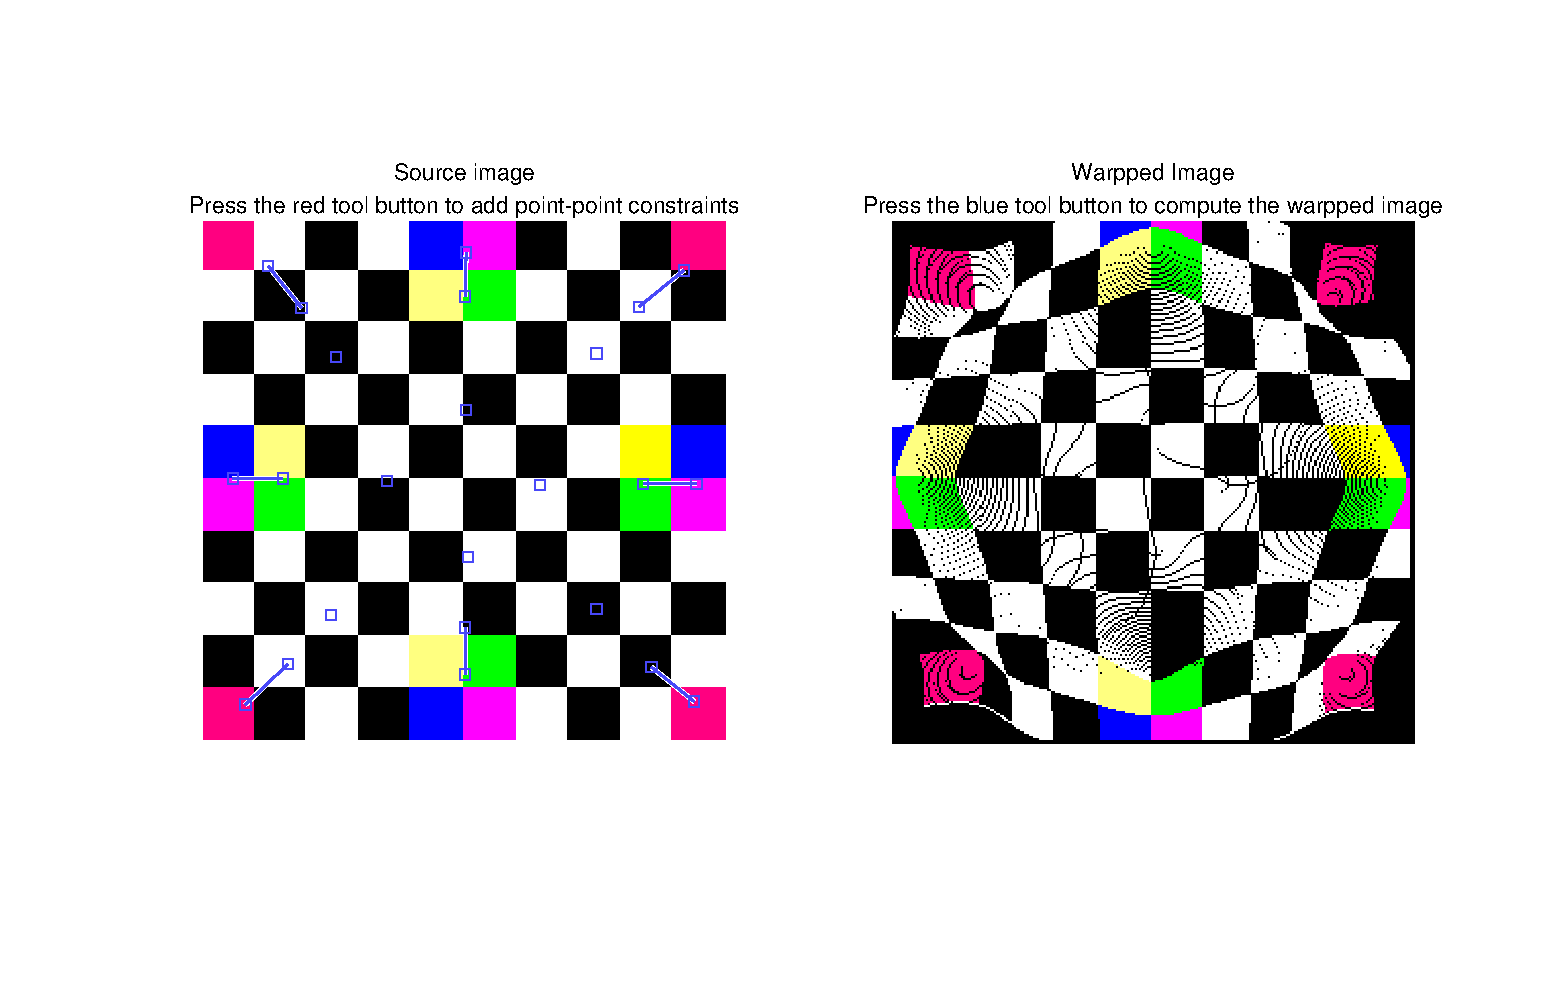
\includegraphics[width=0.5\textwidth]{ResultImage/idw2.pdf}
    }
    \subfigure[RBF]{
        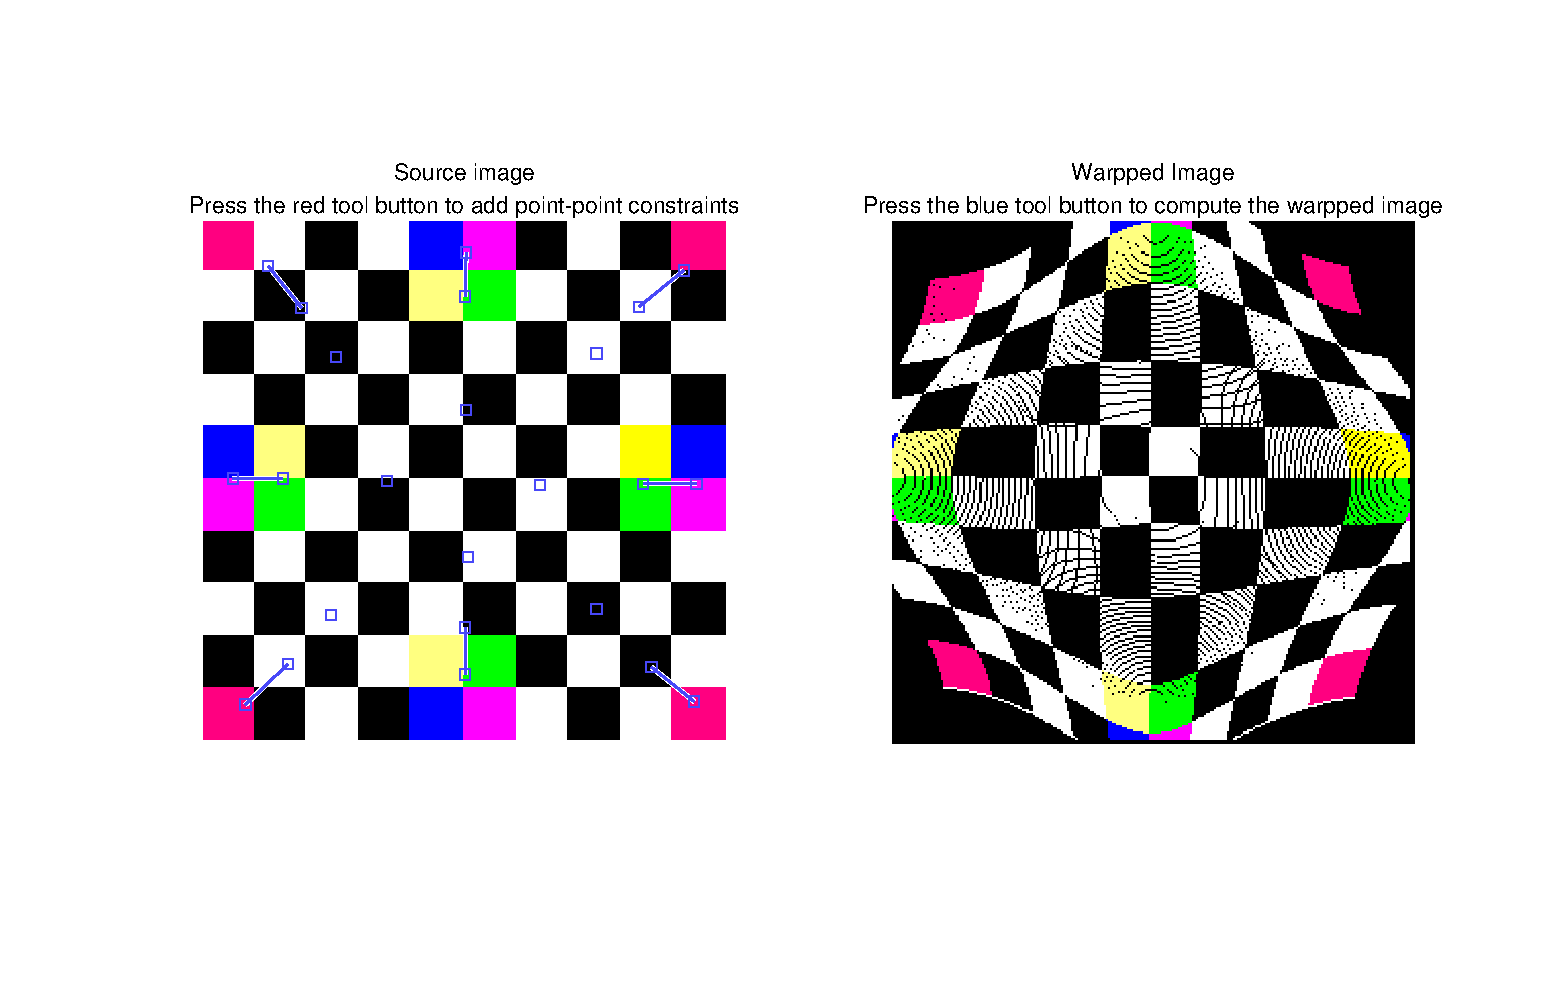
\includegraphics[width=0.5\textwidth]{ResultImage/rbf2.pdf}
    }
    \subfigure[IDW]{
        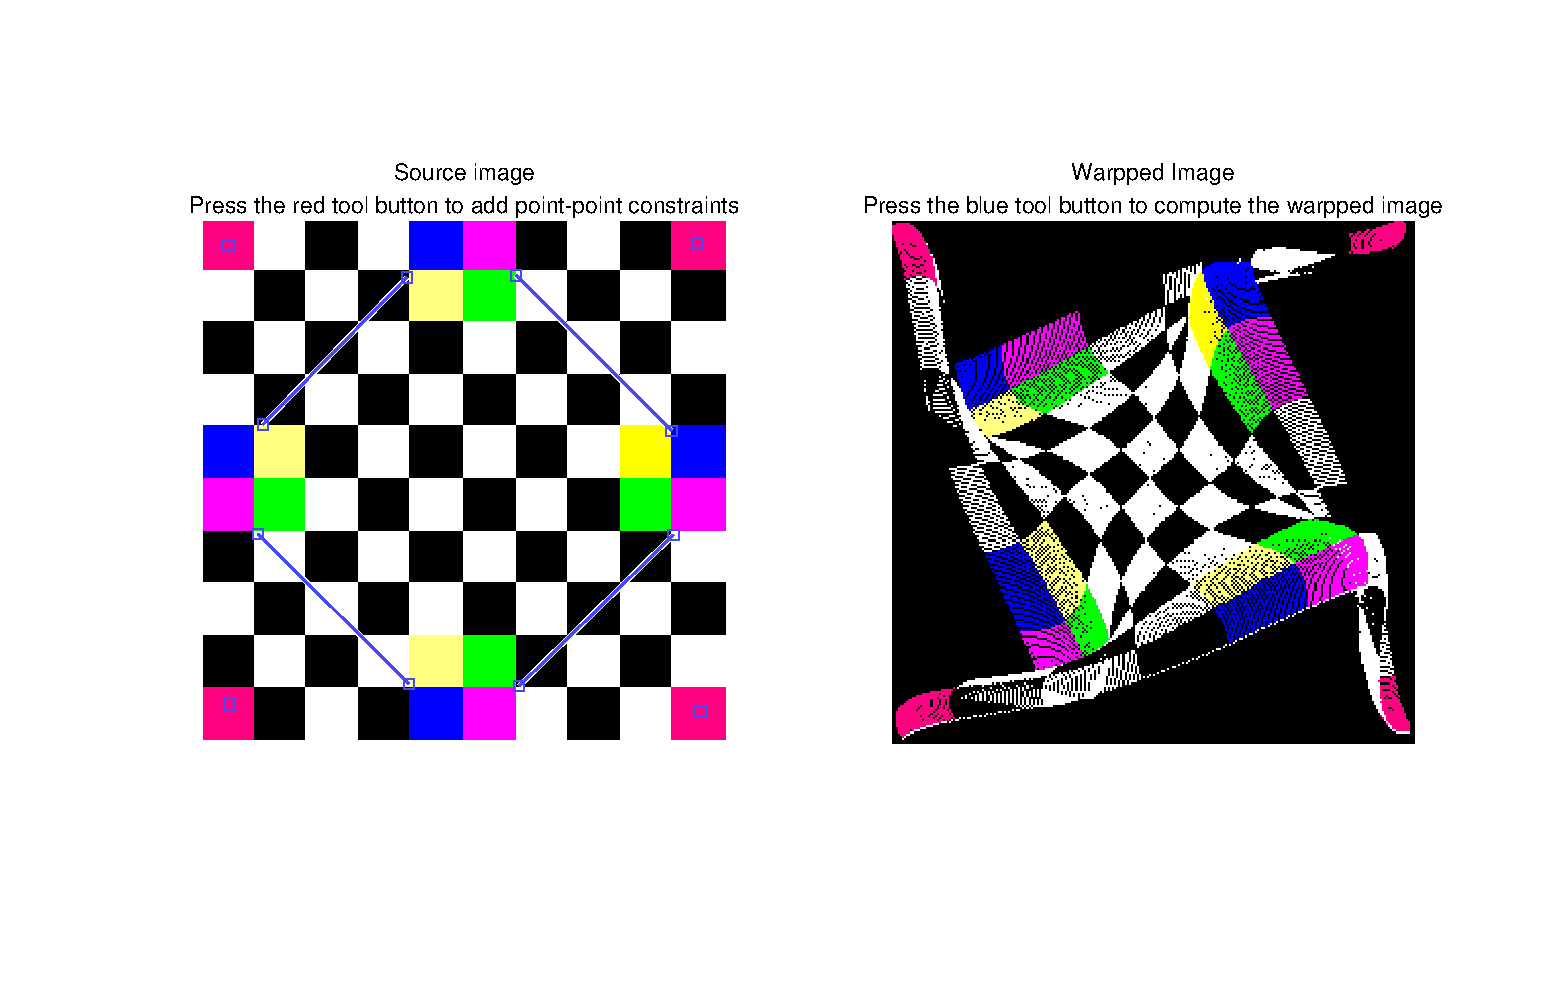
\includegraphics[width=0.5\textwidth]{ResultImage/idw5.pdf}
    }
    \subfigure[RBF]{
        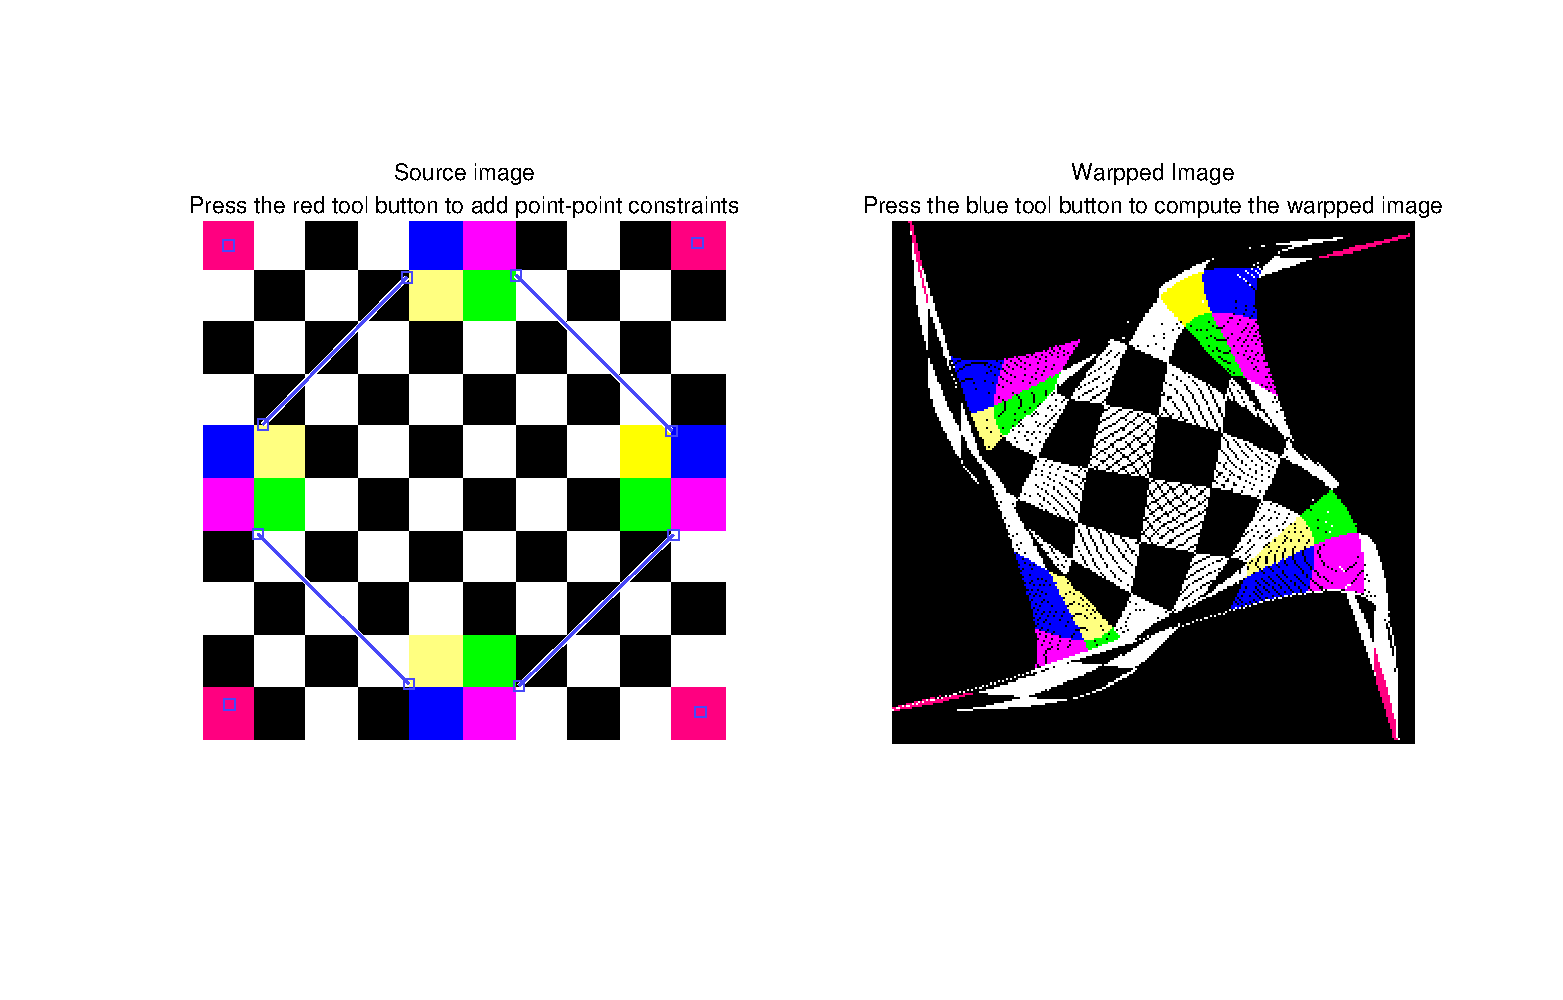
\includegraphics[width=0.5\textwidth]{ResultImage/rbf5.pdf}
    }
\end{figure}

\newpage

\section{Performance Comparisons}
The table below shows the runtime of two algorithm in a $256\times256$-pixel image with different control points numbers in our test.
\begin{table}[H]
    \centering
    \begin{tabular}{|c|ccccc|}
        \hline
        n      & 4        & 8        & 16       & 24       & 32       \\
        \hline
        IDW(s) & 0.947608 & 1.506009 & 3.044657 & 3.725757 & 4.742689 \\
        RBF(s) & 0.297725 & 0.357402 & 0.536027 & 0.549384 & 0.667023 \\
        \hline
    \end{tabular}
\end{table}
we can see in the same image with the same control points, RBF method spent less time. And with the same number of control points, RBF method leads to a more precise result(see figure(a) and(b)).

Also, in the image test, we can see some disadvantages of IDW and RBF. One of them is that we cannot mapping the original image to every pixel of the result image, which causes the black hole or gap in the result image. The other disadvantage is that in some extreme situation, the IDW and RBF will cause the foldover in the result image(see figure (g) and (h)).


\appendix
\section{Code}
All the code of this assignment can be downloaded from \url{https://github.com/mathendy/MS-USTC/tree/master/Code%20Training/matlab-1_assignment}.

\end{document}